% !TeX spellcheck = de_DE
\section{Methodik}
\label{sec:Methodik}

	\subsection{Datensatz}
	\label{ssec:Datensatz}

	    Der für die Modellwahl verwendete Datensatz beinhaltet die logarithmierten relativen Reflexionswerte $-\delta(\lambda)$ bei Wellenlängen zwischen 1400 nm und 2672 nm in einem Abstand von 4 nm sowie die Stoffmengeanteile $y^{(N)}$, $y^{(SOC)}$ und entsprechenden pH-Werte von insgesamt 533 Proben.
	    Informationen über die chemische Zusammensetzung der Probe in den Reflexionswerten im Nahinfrarotbereich sind stark überlagert. \cite{Agelet2010}
	    Aus diesem Grund ist eine sorgfältige Auswahl relevanter Wellenlängen von besonderer Bedeutung für die Erstellung eines zuverlässigen Modells.


	% subsection Datensatz

	\subsection{Statistisches Modell}
	\label{ssec:Statistisches Modell}

	    Sei $n\in\SN$ die Größe des Datensatzes und $k\in\SN$ mit $k< n$ die Anzahl der Wellenlängen im Datensatz.
	    Entsprechend Abschnitt \ref{ssec:Datensatz} definieren wir dann die Einflussgröße $x_{ij}$ als für die $i$te Probe und $j$te Wellenlänge als
	    \[
			x_{ij} \define -\lg \delta_i(\lambda_j)
		\]
		für jedes $i,j\in\SN,i\leq n,j\leq k$.

	    Der Stoffmengenanteil des Stickstoffs  $y^{(N)}$ stellt die Zielgröße unseres späteren Modells dar.
	    Wie definieren hierfür den Vektor $y_i$ den Stoffmengenanteil der $i$ten Probe als den $n$ dimensionalen Vektor
		\[
			 y^{(N)} \define \curvb{y^\m{(N)}_i}
		\]

        Nachdem wir sowohl die Einflussgrößen als auch die Zielgröße für das lineare Modell definiert haben lassen sich diese nun in Zusammenhang bringen.
        Es ist plausibel anzunehmen, die sich sie Zielgröße durch einen Linearkombination der Einflussgrößen beschreiben lässt.
        Hierfür definieren wir zunächst $Y^\m{(N)}$ als einen zufälligen Vektor von $y^\m{(N)}$
        \[
			 \expect Y^\m{(N)} \define \beta_0 + \sum_{j=1}^k{x_{ij}\beta_j}
		\]

		Zudem ist es notwendig eine Variable $\varepsilon^\m{(N)}$ einzuführen welchen den Zufall der Messungen beschreibt.
	    In Matrixschreibweise lässt sich dies als die Designmatrix $\mathbb{X} \in \SR^{n \times (k+1)}$, dem Parametervektor $\beta \in \SR^{k+1}$ und dem stochastisch  verteilten Parameter $\varepsilon^\m{(N)}$ darstellen, sodass gilt,
		\[
			Y^\m{(N)} = \mathbb{X}\beta + \varepsilon^\m{(N)}
		\]
		mit
		\[
			\expect \varepsilon^\m{(N)} = 0, \qquad \cov \varepsilon^\m{(N)} = (\sigma^2)^\m{(N)} \idmat
		\]
		wobei $(\sigma^2)^\m{(N)} \in (0,\infty)$.
		Weiterhin soll angenommen werden, dass $\varepsilon^\m{(N)}$ normalverteilt ist mit
	    \[
			\varepsilon^\m{(N)} \sim \FN \curvb{0,(\sigma^2)^\m{(N)}\idmat}
		\]
	    sodass sich für das Gesamtmodell gilt
		\[
			Y^\m{(N)} \sim \FN \curvb{\mathbb{X}\beta^\m{(N)},(\sigma^2)^\m{(N)} \idmat}
		\]

	% subsection Statistisches Modell

	\subsection{Modellwahl im Falle der NIR-Spektroskopie}
	\label{ssec:mlr}
	Seien $Y\in \rm I\!R^{n}$ die Zielgröße in einem statistischen Modellwahlverfahrens und $\mathbb{X} \in \rm I\!R^{n \times d}$ eine Designmatrix.
	Zur Wahl einer geeigneten Menge von $k$ Einflussparametern auf die Zielgröße $y_i$  wird klassischerweise die Modellwahl über eine hierarchische Aufstellung von linearen Modellen erreicht. Beginnend mit dem minimalen Modell $E(Y_i) = \beta_0$ werden nach und nach neue potenzielle Einflussparameter $x_{ik}$ hinzugefügt. Zu jedem dieser neuen $x_{ik}$ wird dann eine Teststatistik aufgestellt, die darauf hinweist, ob der gewählte Parameter wichtig ist ist oder nicht. Dabei ist die Nullhypothese, dass $x_{ik}$ keinen Einfluss auf die Zielgröße hat: $ H_0 = \beta_k = 0$ und wird abgelehnt, falls $H_1 = \beta_k \neq 0$ zutrifft. 
	Dies wird über die T-Teststatistik erreicht,  wobei für den Fall, dass $H_0$ richtig ist, gilt: 
	\begin{align}
	\frac{\hat{\beta_k}}{\sqrt{\sigma^2(\mathbb{X}^T\mathbb{X})^{-1}_{kk}}} \sim t_{n-(k+1)}.
	\end{align}
	Dieses Verfahren ist vor allem dann besonders gut geeignet, wenn man bereits theoretisch fundierte Annahmen über die Einflussgrößen machen kann.
	Mit diesem Modellwahlverfahren ergeben sich hier allerdings einige Schwierigkeiten, wobei die für unseren Fall besonders schwerwiegenden herausgehoben werden: In dieser Arbeit haben wir es mit einer großen Anzahl potenzieller Einflussvariablen auf dem Nah-Infrarotspektrum zu tun. A priori kann schwer eine inhaltliche Deutung vorgenommen werden, die gewisse Wellenlängen bevorzugt. Daher ist eine hierarchische Modellwahl mit wenigen, theoretisch begründeten Einflussvariablen nicht möglich. Demnach muss in dieser Arbeit die Anzahl der möglichen Einflussgrößen stark erhöht werden und hier bekommen wir ein Problem mit der T-Teststatistik. Es ließen sich sehr viele unterschiedliche Kombinationen von Einflussgrößen aufstellen und in eine hierarchische Form bringen. Doch da wir bei der T-Teststatistik ein \underline{zufälliges} Intervall konstruieren, gegen das unsere Hypothese getestet wird, wird die Wahrscheinlichkeit bei oft wiederholten Tests fälschlicherweise die Nullhypothese abzulehnen mit Anzahl der Versuchen immer größer. An ein automatisiertes Modellwahlverfahren, das in dieser Arbeit von Vorteil ist, ist also mittels des T-Tests nicht zu erreichen \cite{Schumacher.2019}.
	Stattdessen bietet sich eine Modellwahl basierend auf dem erwarteten Prognosefehler ("sum of prediction squared error", SPSE) an: 
	\begin{align}
		SPSE := E(\sum_{i=1}^{n} (Y_{i+n} - x_{i}^{(M)}\hat{\beta_i}^{((M)})^2)
	\end{align}
	Hierbei sind die Werte in $Y_{i+n}$ neue Beobachtungen zum Erwartungsvektor $x_i$ und $x_{i}^{(M)}\hat{\beta_i}^{((M)}$ ist sind die Prognosewerte aus dem zu testenden Modell $M$. 
	Der Prognosefehler lässt sich in 3 Terme zerlegen: Einen irreduzierbaren Prognosefehler, der unabhängig von dem momentan betrachteten Modell ist, einen Biasterm, der die Abweichung des aktuellen Modells $M$ vom Prognosemodell als Summe der quadrierten Prognose-Verzerrungen anzeigt und einen Varianzterm, der die Ungenauigkeiten widerspiegelt, die sich aus der Schätzung von $p = (|M|+1)$ unbekannten Parametern ergibt:
	\begin{align}
	SPSE^{(M)} = n\sigma_{full}^2 + p\sigma_{full}^2 + (bias^{(M)})^2
	\end{align},
	Der SPSE lässt sich über unterschiedliche Wege berechnen / abschätzen, mithilfe neuer Beobachtungen (1), (wiederholter) Zerlegung der Ursprungsdaten in Test- und Trainingsdaten (Kreuzvalidierung) (2) oder mittels Schätzung basierend auf der Residuenquadratsumme ("residual squared sum", RSS), hier im Vergleich zu o.g. SPSE:

	\begin{align}
	RSS^{(M)} := \sum_{i=1}^{n} E (Y_{i} - \hat{Y_i}^{(M)})^2
	\end{align}
	\begin{align}
	SPSE^{(M)} := \sum_{i=1}^{n} E (Y_{i+n} - \hat{Y_i}^{(M)})^2
	\end{align}
	Es kann gezeigt werden, dass RSS den Wert von SPSE systematisch unterschätzt, dass diese Unterschätzung jedoch behoben werden kann, indem für alle Modelle die Varianzschätzung aus dem maximalen Modell verwendet wird\cite{Schumacher.2019}: 
	\begin{align}
	SPSE^{(M)} := RSS^{(M)} + 2 \tilde{\sigma}_{full} ^2 (k+1)
	\end{align}
	Die Minimierung des SPSE entspricht der Minimierung des Mallow's Cp- Kriteriums, das für die folgenden Analysen getestet werden soll. Dabei gilt:
	\begin{align}
	Cp^{(M)} = \frac{1}{\sigma_{full}^2} \sum_{i=1}^{n} (y_i - \hat{y_i}^{(M)})^2 - n + 2(k+1)
	\end{align}
	
	

	\subsection{Modellselektion}
	\label{ssec:modellselektion}
	Das erste Ziel dieser Arbeit ist es, diejenigen Wellenlängen herauszufinden, deren Reflektionswert der Nahinfrarot-Spektroskopie einen Einfluss auf den Stickstoffgehalt des Untergrunds hat. Dazu wurden mehrere Selektionsverfahren verglichen. Zunächst wurde die erste Ableitung der Wellenlängen verwendet, um die \underline{Veränderungen} der Reflektionswerte nach Wellenlängen zu untersuchen. Des Weiteren wurden die Daten nach Wellenlängen-Bereichen untersucht, in denen die größte Variabilität zu finden ist. Die untersuchten Modelle sind in folgender Tabelle zu 
	\begin{table}
		
	\end{table}
	
	
	\begin{figure*}
		\label{Wellenlängen_erste_Ableitung}
		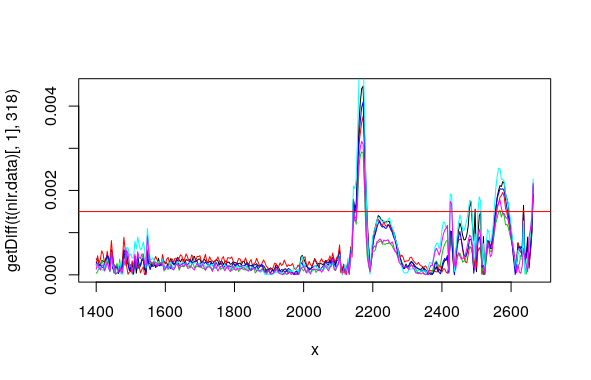
\includegraphics[width=\textwidth]{img/wave_1dev.png}
		\caption{Ableitungen der Wellenlängen von fünf zufälligen Spektren}
	\end{figure*}
	Über dieses maximale Modell wurde nun mittels Mallows Cp ein bestes Modell(siehe Kapitel \ref{ssec:mlr}) berechnet.
	
	\subsection{SPSE-Vergleich}
	Das zweite Ziel dieser Arbeit ist der Vergleich des SPSE-Wertes für das aus \ref{ssec:modellselektion} gewonnene Idealmodell und der SPSE Schätzung über Mallows Cp, welches auf zufällig gezogene Spektren angewandt wurde. 
	Zunächst 

	
	% subsection model-validation
	
	%\subsection{Assessment by Simulation}
	%\label{ssec:simulation}
	
		
		

